\documentclass[tikz,border=8pt]{standalone}
% Shared UMM figure style (journal-consistent palette + line weights)
\usepackage{tikz}
\usepackage{pgfplots}
\pgfplotsset{compat=1.18}
\usetikzlibrary{arrows.meta,calc,positioning,decorations.pathmorphing,patterns,shapes.geometric,fit,backgrounds}
% Palette: grayscale + single accent (deep teal)
\definecolor{ummAccent}{HTML}{0B6E6E}
\definecolor{ummAccentLight}{HTML}{4A9B9B}
\definecolor{ummDark}{HTML}{1A1A1A}
\definecolor{ummGray}{HTML}{555555}
\definecolor{ummLightGray}{HTML}{AAAAAA}
\definecolor{ummFill}{HTML}{E8F2F2}
\definecolor{ummGas}{HTML}{C45C26}
\definecolor{ummGasLight}{HTML}{F0C4A8}
\definecolor{ummGalaxy}{HTML}{2C3E50}
\definecolor{ummLens}{HTML}{0B6E6E}
\pgfplotsset{
  umm axis/.style={
    axis lines=left,
    axis line style={ummDark, line width=0.8pt},
    tick style={ummDark, line width=0.6pt},
    tick label style={font=\footnotesize, ummDark},
    label style={font=\small, ummDark},
    title style={font=\small\bfseries, ummDark},
    grid=both,
    major grid style={ummLightGray, opacity=0.35, line width=0.3pt},
    minor grid style={ummLightGray, opacity=0.15, line width=0.2pt},
    every axis plot/.append style={line width=1.3pt},
    legend style={font=\footnotesize, draw=ummLightGray, fill=white, fill opacity=0.92, text opacity=1},
    clip=false,
  },
}
\newcommand{\ummLineW}{1.25pt}
\newcommand{\ummLineWthin}{0.9pt}
\tikzset{
  umm arr/.style={-{Latex[length=2.2mm,width=1.6mm]}},
}

\begin{document}
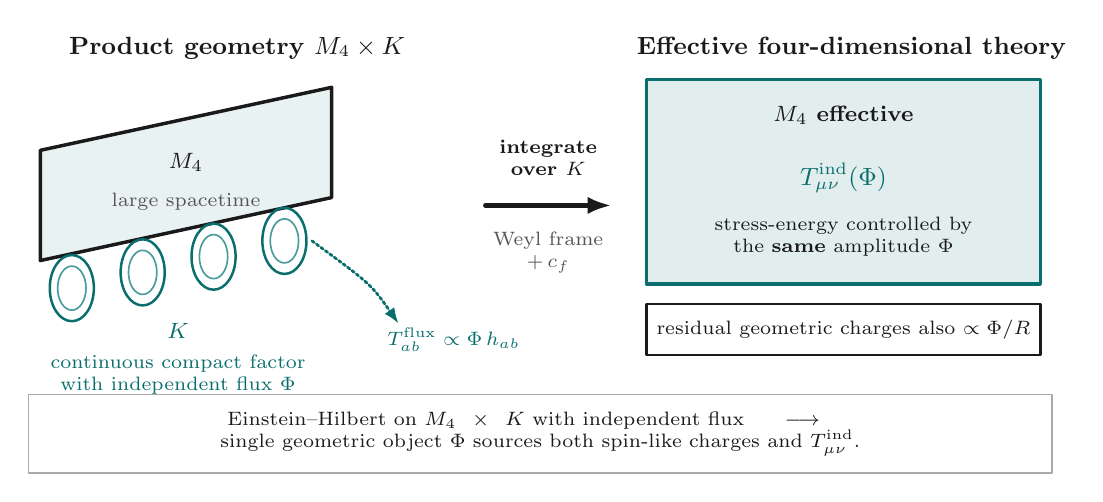
\begin{tikzpicture}[font=\small, line cap=round, line join=round]
  % ===== Left block: M4 x K =====
  \node[font=\bfseries\small, ummDark] at (2.8, 5.55) {Product geometry $M_4\times K$};

  % Spacetime slab M4
  \fill[ummFill] (0.3,2.85) -- (4.0,3.65) -- (4.0,5.05) -- (0.3,4.25) -- cycle;
  \draw[ummDark, line width=\ummLineW]
    (0.3,2.85) -- (4.0,3.65) -- (4.0,5.05) -- (0.3,4.25) -- cycle;
  \node[font=\footnotesize\bfseries, ummDark] at (2.15,4.1) {$M_4$};
  \node[font=\scriptsize, ummGray] at (2.15,3.6) {large spacetime};

  % Compact fiber K
  \foreach \x/\y in {0.7/2.5, 1.6/2.7, 2.5/2.9, 3.4/3.1} {
    \draw[ummAccent, line width=\ummLineWthin] (\x,\y) ellipse (0.28 and 0.42);
    \draw[ummAccentLight, line width=0.6pt] (\x,\y) ellipse (0.18 and 0.28);
  }
  \node[font=\footnotesize\bfseries, ummAccent] at (2.05,1.95) {$K$};
  \node[font=\scriptsize, ummAccent, align=center] at (2.05,1.4)
    {continuous compact factor\\with independent flux $\Phi$};

  % Flux annotation on K
  \draw[ummAccent, densely dotted, line width=1.0pt,
        -{Latex[length=2mm]}]
    (3.75,3.1) .. controls (4.5,2.55) .. (4.85,2.05);
  \node[font=\scriptsize, ummAccent, align=left] at (5.55,1.85)
    {$T_{ab}^{\mathrm{flux}}\propto\Phi\,h_{ab}$};

  % ===== Arrow: integrate over K =====
  \draw[ummDark, line width=1.5pt, -{Latex[length=3mm,width=2.2mm]}]
    (5.95,3.55) -- (7.55,3.55);
  \node[font=\scriptsize\bfseries, ummDark, align=center] at (6.75,4.15)
    {integrate\\over $K$};
  \node[font=\scriptsize, ummGray, align=center] at (6.75,2.95)
    {Weyl frame\\$+\,c_f$};

  % ===== Right block: effective 4D =====
  \node[font=\bfseries\small, ummDark] at (10.6, 5.55) {Effective four-dimensional theory};

  \fill[ummAccent!12] (8.0,2.55) -- (13.0,2.55) -- (13.0,5.15) -- (8.0,5.15) -- cycle;
  \draw[ummAccent, line width=\ummLineW]
    (8.0,2.55) rectangle (13.0,5.15);
  \node[font=\footnotesize\bfseries, ummDark] at (10.5,4.7) {$M_4$ effective};
  \node[font=\small, ummAccent, align=center] at (10.5,3.9)
    {$T_{\mu\nu}^{\mathrm{ind}}(\Phi)$};
  \node[font=\scriptsize, ummDark, align=center] at (10.5,3.15)
    {stress-energy controlled by\\the \textbf{same} amplitude $\Phi$};

  % Residual charges link
  \draw[ummDark, line width=\ummLineWthin]
    (8.0,1.65) rectangle (13.0,2.3);
  \fill[white] (8.02,1.67) rectangle (12.98,2.28);
  \node[font=\scriptsize, ummDark] at (10.5,1.97)
    {residual geometric charges also $\propto\Phi/R$};

  % Bottom flow summary (full width, no overflow)
  \draw[ummLightGray, line width=0.6pt] (0.15,0.15) rectangle (13.15,1.15);
  \fill[white] (0.17,0.17) rectangle (13.13,1.13);
  \node[font=\scriptsize, ummDark, align=center, text width=12.7cm] at (6.65,0.65)
    {Einstein--Hilbert on $M_4\times K$ with independent flux
     $\;\longrightarrow\;$
     \mbox{single} geometric object $\Phi$ sources both spin-like charges and $T_{\mu\nu}^{\mathrm{ind}}$.};
\end{tikzpicture}
\end{document}
